\documentclass[a4paper]{article}
\usepackage{amsfonts}
\usepackage{amsmath}
\usepackage{amssymb}
\usepackage{graphicx}
\begin{document}

\noindent \large Auteur: Anass Hamzaoui \\
\noindent \large Studierichting: Informatica \\
\noindent \large Oefeningenreeks 5F nr. 3.2 \\
\medskip
\normalsize

$\left|\begin{array}{ll}
    & r_1 = \cos\theta: \text{ cirkel, middelpunt } \left(\dfrac{1}{2}, 0\right), \text{ straal } \dfrac{1}{2} \\
    
    & r_2 = 1 - \cos\theta: \text{ cardio\"{i}de, geori\"{e}nteerd naar links} \\
    
    & r_1 = r_2 \implies \cos\theta = 1 - \cos\theta \implies \cos\theta = \dfrac{1}{2} \implies \theta = \pm\dfrac{\pi}{3}, \quad r = \dfrac{1}{2} \\
\end{array}\right.$ \\

Grafiek: \\
\begin{figure}[h]
\centering
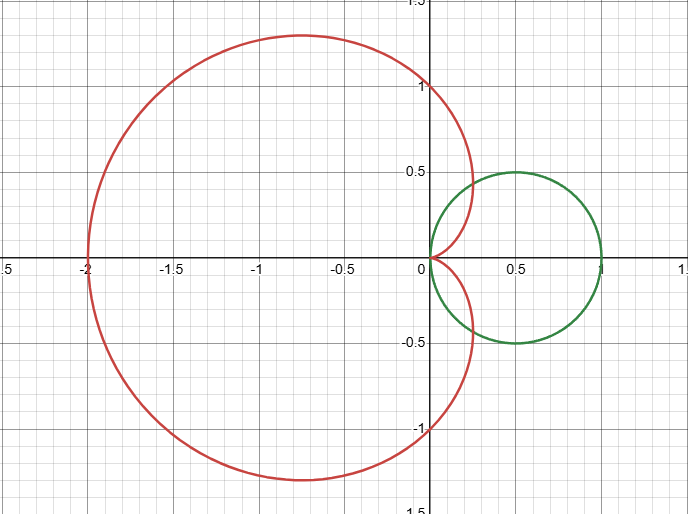
\includegraphics[width=8cm]{5F-3.2-anass.hamzaoui.INF.png}
\end{figure}

$\begin{array}{ll}
S &= 2\left(\dfrac{1}{2}\displaystyle\int_0^{\pi/3}(1-\cos\theta)^2    d\theta + \dfrac{1}{2}\displaystyle\int_{\pi/3}^{\pi/2}\cos^2\theta    d\theta\right) \\

&= \displaystyle\int_0^{\pi/3}(1 - 2\cos\theta + \cos^2\theta)    d\theta + \displaystyle\int_{\pi/3}^{\pi/2}\cos^2\theta    d\theta \\

&= \displaystyle\int_0^{\pi/3}\left(\dfrac{3}{2} - 2\cos\theta + \dfrac{1}{2}\cos 2\theta\right)d\theta + \displaystyle\int_{\pi/3}^{\pi/2}\dfrac{1+\cos 2\theta}{2}    d\theta \\

&= \left[\dfrac{3}{2}\theta - 2\sin\theta + \dfrac{\sin 2\theta}{4}\right]_0^{\pi/3} + \left[\dfrac{\theta}{2} + \dfrac{\sin 2\theta}{4}\right]_{\pi/3}^{\pi/2} \\

&= \left(\dfrac{\pi}{2} - \sqrt{3} + \dfrac{\sqrt{3}}{8}\right) + \left(\dfrac{\pi}{4} - \dfrac{\pi}{6} - \dfrac{\sqrt{3}}{8}\right) \\

&= \dfrac{\pi}{2} - \dfrac{7\sqrt{3}}{8} + \dfrac{\pi}{12} - \dfrac{\sqrt{3}}{8} \\

&= \dfrac{7\pi}{12} - \sqrt{3} \\
\end{array}$

\begin{thebibliography}{999}
    %\bibitem{a} Referentie
\end{thebibliography}
\end{document}